\documentclass[11pt,a4j]{jsarticle}
\title{ゆらぎ}
\author{1413176 三村幸祐}
\date{2016/11/30 \, 2016/12/7}
\usepackage{booktabs}
\usepackage[dvipdfmx,hiresbb]{graphicx}
%\pagestyle{empty}

\begin{document}
  
% \tableofcontents
  
% \newpage
  
 \section{目的}
  実際の物理実験の測定において「ゆらぎ」の現象は必ず生じている。このゆらぎは様々な物理的要因に由来し、それらは定量的に扱うことができる。
  
  今回はあえてアンプでゆらぎを増幅させ、その要因となる物理理論からボルツマン定数$k_B$u、及び電気素量$e$を測定する。
  
  
 \section{原理}
   
   \subsection{増幅器の特性と雑音指数$F$}
  今回は増幅器を用いてあえてゆらぎを増幅して、その挙動を調べる。しかし増幅器も内部の抵抗成分などにより増幅率の周波数特性が存在する。つまり電圧増幅率$G$には
  \begin{equation}
  G = G(f)
  \end{equation}
  というように周波数依存性がある。今回は一定の入力電圧$v_i$に対する増幅を見ていくため、その周波数依存特性の曲線の生成する面積$S$に対して成り立つ
  \begin{equation}
  S = v_i^2 \int G^2 (f) df
  \end{equation}
  という関係を用いて
  \begin{eqnarray}
  <V^2> &=& \frac{<v^2>}{\Delta f} \int G^2 (f) df \\
  \frac{<v^2>}{\Delta f} &=& \frac{<V^2> v_i^2}{S} \label{eq:13}
  \end{eqnarray}
  となる。
   
   \subsection{熱雑音とボルツマン定数}
   抵抗にはその両端に自由電子の熱的運動に起因する雑音が生じる。この雑音を熱雑音と呼ぶがその熱雑音電圧$v$として、抵抗$R$電圧を測定する帯域幅を$\Delta f$、抵抗の温度を$T$、ボルツマン定数を$k_B$とすると
   \begin{equation}
   <v^2> = 4k_B TR \Delta f
   \label{eq:1}
   \end{equation}
   としてvの2乗平均は評価される。この式(\ref{eq:1})はナイキストの熱雑音の式という。
   
   ただし今回は上記のように増幅器の特性を考慮しなければならないため、周波数幅$\Delta f$と電圧平均は定義を式(\ref{eq:13})のように変える必要がある。
   したがって実験的には
   \begin{eqnarray}
   <V^2> &=& \frac{4k_B TS}{v_i^2} R \label{eq:18} \\
   log<V^2> &=& log(R) - log(\frac{v_i^2}{S} \frac{1}{4k_B T}) \label{eq:17}
   \end{eqnarray}
   という式を用いてデータを処理する。今回は複数の$R$に対して$<V^2>$を測定することでボルツマン定数を求めるのに使用する。
   
   \subsection{散射雑音}
   
   フォトダイオードなど、光-電圧変換の際に生じるゆらぎを散射雑音といい、ここではそれを調べる。
   抵抗Rと直列につないだフォトダイオードにフィラメントなどによる光を入射させた場合、測定した電流ゆらぎの2乗平均値$<I^2> = \frac{<V^2>}{R^2}$と平均電流$<i>$の間には
   \begin{equation}
   <I^2> = \frac{<i_n^2>}{\Delta f} \int G^2 (f) df = \frac{<i_n^2>}{\Delta f} \frac{S}{v_i^2}
   \end{equation}
   の関係が成り立つ。また電気素量は
   \begin{equation}
   e = <I^2> \frac{v_i^2}{S} \frac{1}{2<i>}
   \label{eq:19}
   \end{equation}
   とかけるため、対数表記にして
   \begin{equation}
   log<I^2> = log<i> - log(\frac{v_i^2}{S} \frac{1}{2e})
   \label{eq:20}
   \end{equation}
   というグラフを実験から得ることができる。この切片から電気素量を計算していく。
   
  
 \section{測定手順}
   \subsection{増幅器とフィルターの増幅特性の測定}
   \begin{enumerate}
   \item 抵抗分割器を介して発振器出力をプリアンプのA入力端子に、プリアンプの出力をバンドパスフィルターの入力に、バンドパスフィルターの出力をオシロスコープにそれぞれ接続。
   \item 入力電圧$v_i = 1.01 * 10^{-4}$Vの一定にし、周波数fを50Hz-20kHzの範囲で変化させ、オシロスコープで正弦波の$V_{pp}$値を測定。
   \end{enumerate}
   
   \subsection{ボルツマン定数の測定}
   
   \begin{enumerate}
   \item 可変抵抗をプリアンプの入力に、プリアンプの出力をバンドパスフィルターを通してオシロスコープに接続。
   \item 入力である可変抵抗の抵抗値を変えながら、$<V^2>$の値を測定。
   \end{enumerate}
   
   \subsection{電気素量$e$の測定}
   
   \begin{enumerate}
   \item 「ボルツマン定数の測定」の入力を可変抵抗から出力を変化できるフィラメントに対するフォトダイオードの検波装置に切り替えた。なお、検波装置には抵抗Rが直列に配置されており、オシロスコープには抵抗にかかる電圧波形が表示されるようになっている。
   \item フィラメントの光の出力を変えながら、検波回路に流れる平均電流$<i>$と電圧ゆらぎの2乗平均値$<V^2>$を測定。
   \end{enumerate}
   
  
  
  
 \section{結果と考察}
   \subsection{増幅器とフィルターの増幅特性の測定}
   
   図\ref{fig:1_f-v}に増幅器の周波数特性のデータを示す。
   
   \begin{figure}[htbp]
  \centering
  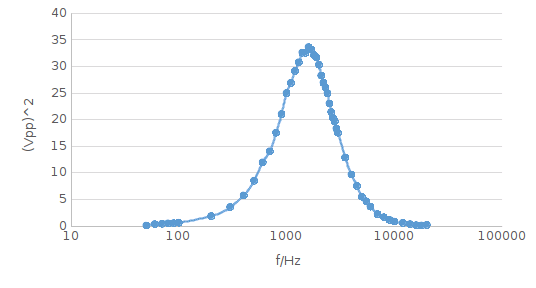
\includegraphics[width=8cm,clip]{1_f-v.png}
  \caption{増幅された電圧波形振幅の周波数依存性}
  \label{fig:1_f-v}
 \end{figure}%
   
   このグラフの面積$S$を台形求積により計算すると、
   \begin{equation}
   S = 32.6 kV^2 Hz \nonumber
   \end{equation}
   となる。ただし、この面積はあるデータのy座標に、そのx座標と次のデータのx座標との差の積をすべてのデータに対して足し合わせたものである。
   
   したがって
   \begin{equation}
   \frac{v_i^2}{S} = 3.1 * 10^{-13} s \nonumber
   \end{equation}
   となる。この値はその増幅率の特性を示すひとつの評価方法であり、今後使用する。
   
   \subsection{ボルツマン定数の測定}
   
   測定した熱雑音の波形観測例を図\ref{fig:wave1}に示す。なお、以降の電圧値などは、波形の最も離れたpp値をとっている。
   
   \begin{figure}[htbp]
  \centering
  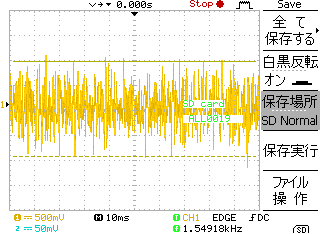
\includegraphics[width=8cm,clip]{A0019DS.png}
  \caption{熱雑音の測定波形例}
  \label{fig:wave1}
 \end{figure}%
   
   図\ref{fig:2_before},\ref{fig:2_after}にそれぞれ2乗平均電圧と抵抗値の両対数グラフ、またその中から傾きが一定になる領域を抜粋したものを載せる。
   \begin{figure}[htbp]
  \centering
  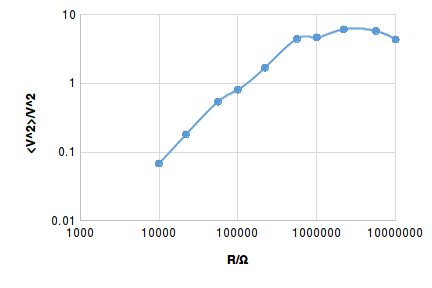
\includegraphics[width=8cm,clip]{2_before.png}
  \caption{2乗平均電圧と抵抗値の両対数グラフ}
  \label{fig:2_before}
 \end{figure}%
   
   \begin{figure}[htbp]
  \centering
  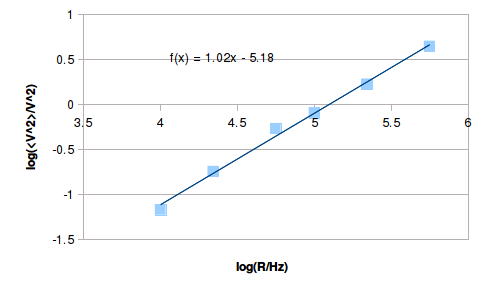
\includegraphics[width=8cm,clip]{2_after.png}
  \caption{2乗平均電圧と抵抗値の抜粋}
  \label{fig:2_after}
 \end{figure}%
   
   図\ref{fig:2_after}と式(\ref{eq:17})の関係によりボルツマン定数が以下のように定まる。
   \begin{equation}
   k_B = 1.7 * 10^{-21} J/K \nonumber \\
   \end{equation}
   ここで室温が26度であったことと、抵抗内部の温度は室温より1度程度高いであろうという予想から抵抗の温度は300Kとしている。
   
   また式(\ref{eq:18})を用いてボルツマン定数の不確かさを求めることを考える。電気測定器による測定値の不確かさは最小目盛$\pm$1、温度の不確かさは$\pm$0.1Kとすると
   \begin{eqnarray}
   \frac{\Delta k_B}{k_B} &=& \sqrt{(2\frac{\Delta v_i}{v_i})^2 + (\frac{\Delta <V^2>}{<V^2>})^2 + (\frac{\Delta T}{T})^2 + (\frac{\Delta S}{S})^2 + (\frac{\Delta R}{R})^2} \nonumber \\
   \Delta k_B &=& 2 * 10^{-22} J/K \nonumber
   \end{eqnarray}
   となる。ただしここで$\frac{\Delta S}{S}$は、図\ref{fig:1_f-v}より$S$を台形求めた場合は傾きの変化量が最も大きい区間でその実際の面積との誤差が大きくなるため、頂点を含む区画の実際の曲線からの台形の差分を$\Delta S$、その区間の台形の面積を$S$としている。そのため$\frac{\Delta S}{S}$比を最も大きくなるように見積もっている。
   
   ここでボルツマン定数の測定値と文献値[1]を以下に比較する。
   \begin{eqnarray}
   k_B \pm \Delta k_B &=& (1.7 \pm 0.2) * 10^{-21} J/K \nonumber \\
   k_B(文献値) &=& 1.4 * 10^{-23} J/K \nonumber
   \end{eqnarray}
   これをみると今回のボルツマン定数の測定値は文献値と、不確かさの幅を考えても全く異なっている。桁が2桁ずれていることがわかる。これは台形求積法による$S$の見積りが小さくなったために、$<V^2> - R$グラフの切片の絶対値に対して$k_B$が大きくなってしまったものと考えられる。対数グラフで数字が違っている点で、桁が多少異なっていることもわかる。
   
   \subsection{電気素量$e$の測定}
   
   測定した散射雑音の波形観測例を図\ref{fig:wave2}に示す。なお、以降の$<I^2> = \frac{<V^2>}{R^2}$の電圧値などは、波形の最も離れたpp値をとっている。
   
   \begin{figure}[htbp]
  \centering
  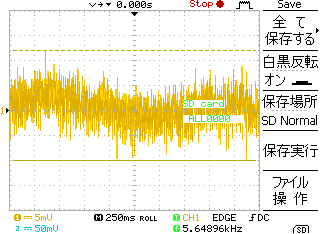
\includegraphics[width=8cm,clip]{A0000DS.png}
  \caption{散射雑音の波形観測例}
  \label{fig:wave2}
 \end{figure}%
   
   測定した電流ゆらぎの2乗平均値と平均電流の両対数グラフを図\ref{fig:3}に示す。
   \begin{figure}[htbp]
  \centering
  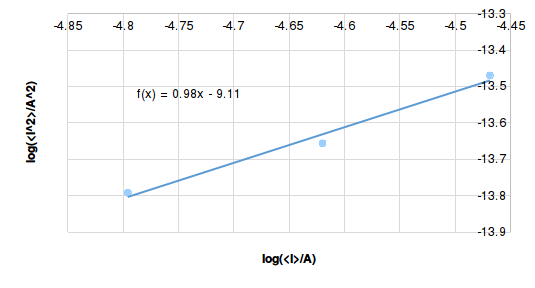
\includegraphics[width=8cm,clip]{3.png}
  \caption{電流ゆらぎの2乗平均と平均電流の両対数グラフ}
  \label{fig:3}
 \end{figure}%
   
   このグラフと式(\ref{eq:20})から、電気素量の測定値は
   \begin{equation}
   e = 1.2 * 10^{-22} C \nonumber \\
   \end{equation}
   となることがわかる。さらにその不確かさは、式(\ref{eq:19})から
   \begin{eqnarray}
   \frac{\Delta e}{e} &=& \sqrt{(\frac{\Delta <I^2>}{<I^2>})^2 + (2\frac{\Delta v_i}{v_i})^2 + (\frac{\Delta S}{S})^2 + (\frac{\Delta <i>}{<i>})^2} \nonumber \\
   \Delta e &=& 1 * 10^{-23} C \nonumber
   \end{eqnarray}
   となる。
   
   以下に電気素量の測定値と文献値[1]を比較する。
   \begin{eqnarray}
   e \pm \Delta e &=& (1.2 \pm 0.1) * 10^{-22} C \nonumber \\
   e(文献値) &=& 1.6 * 10^{-19} C \nonumber
   \end{eqnarray}
   ここでも電気素量は測定値と文献値が3桁ほど異なる(ボルツマン定数では2桁)。これより先述の「ボルツマン定数の測定」の項目との共通項から見ても、$S$の見積りが小さくなってしまっているという点が確かめられる。さらに今回は$<i>$の読み取り精度が低いことによる不確かさの大きさも、電気素量の測定値と文献値の差異の拡大に寄与していると考えられる。
  
  
 \section{参考文献}
  [1]理科年表平成28年,p375
  
  
\end{document}